\section{Übersicht Maschinentechnik}

\subsection{Konstruktion mechanische Komponenten}
Die Konstruktion besteht hauptsächlich aus Aluminium-Blechteilen. Einige 
Komponenten müssen aus konstruktiven Gründen als Frästeile ausgeführt werden.
Um ein geringeres Gewicht zu 
erreichen, werden die Blechteile mit Aussparungen an nicht erforderlichen 
Flächen versehen. Da dies eine Schwächung der Stabilität mit sich bringt werden die Aussparungen, wie im Flugzeugbau üblich, mit gebogenen Innenkanten ausgeführt.

\begin{figure}[h!]          
	\centering             
	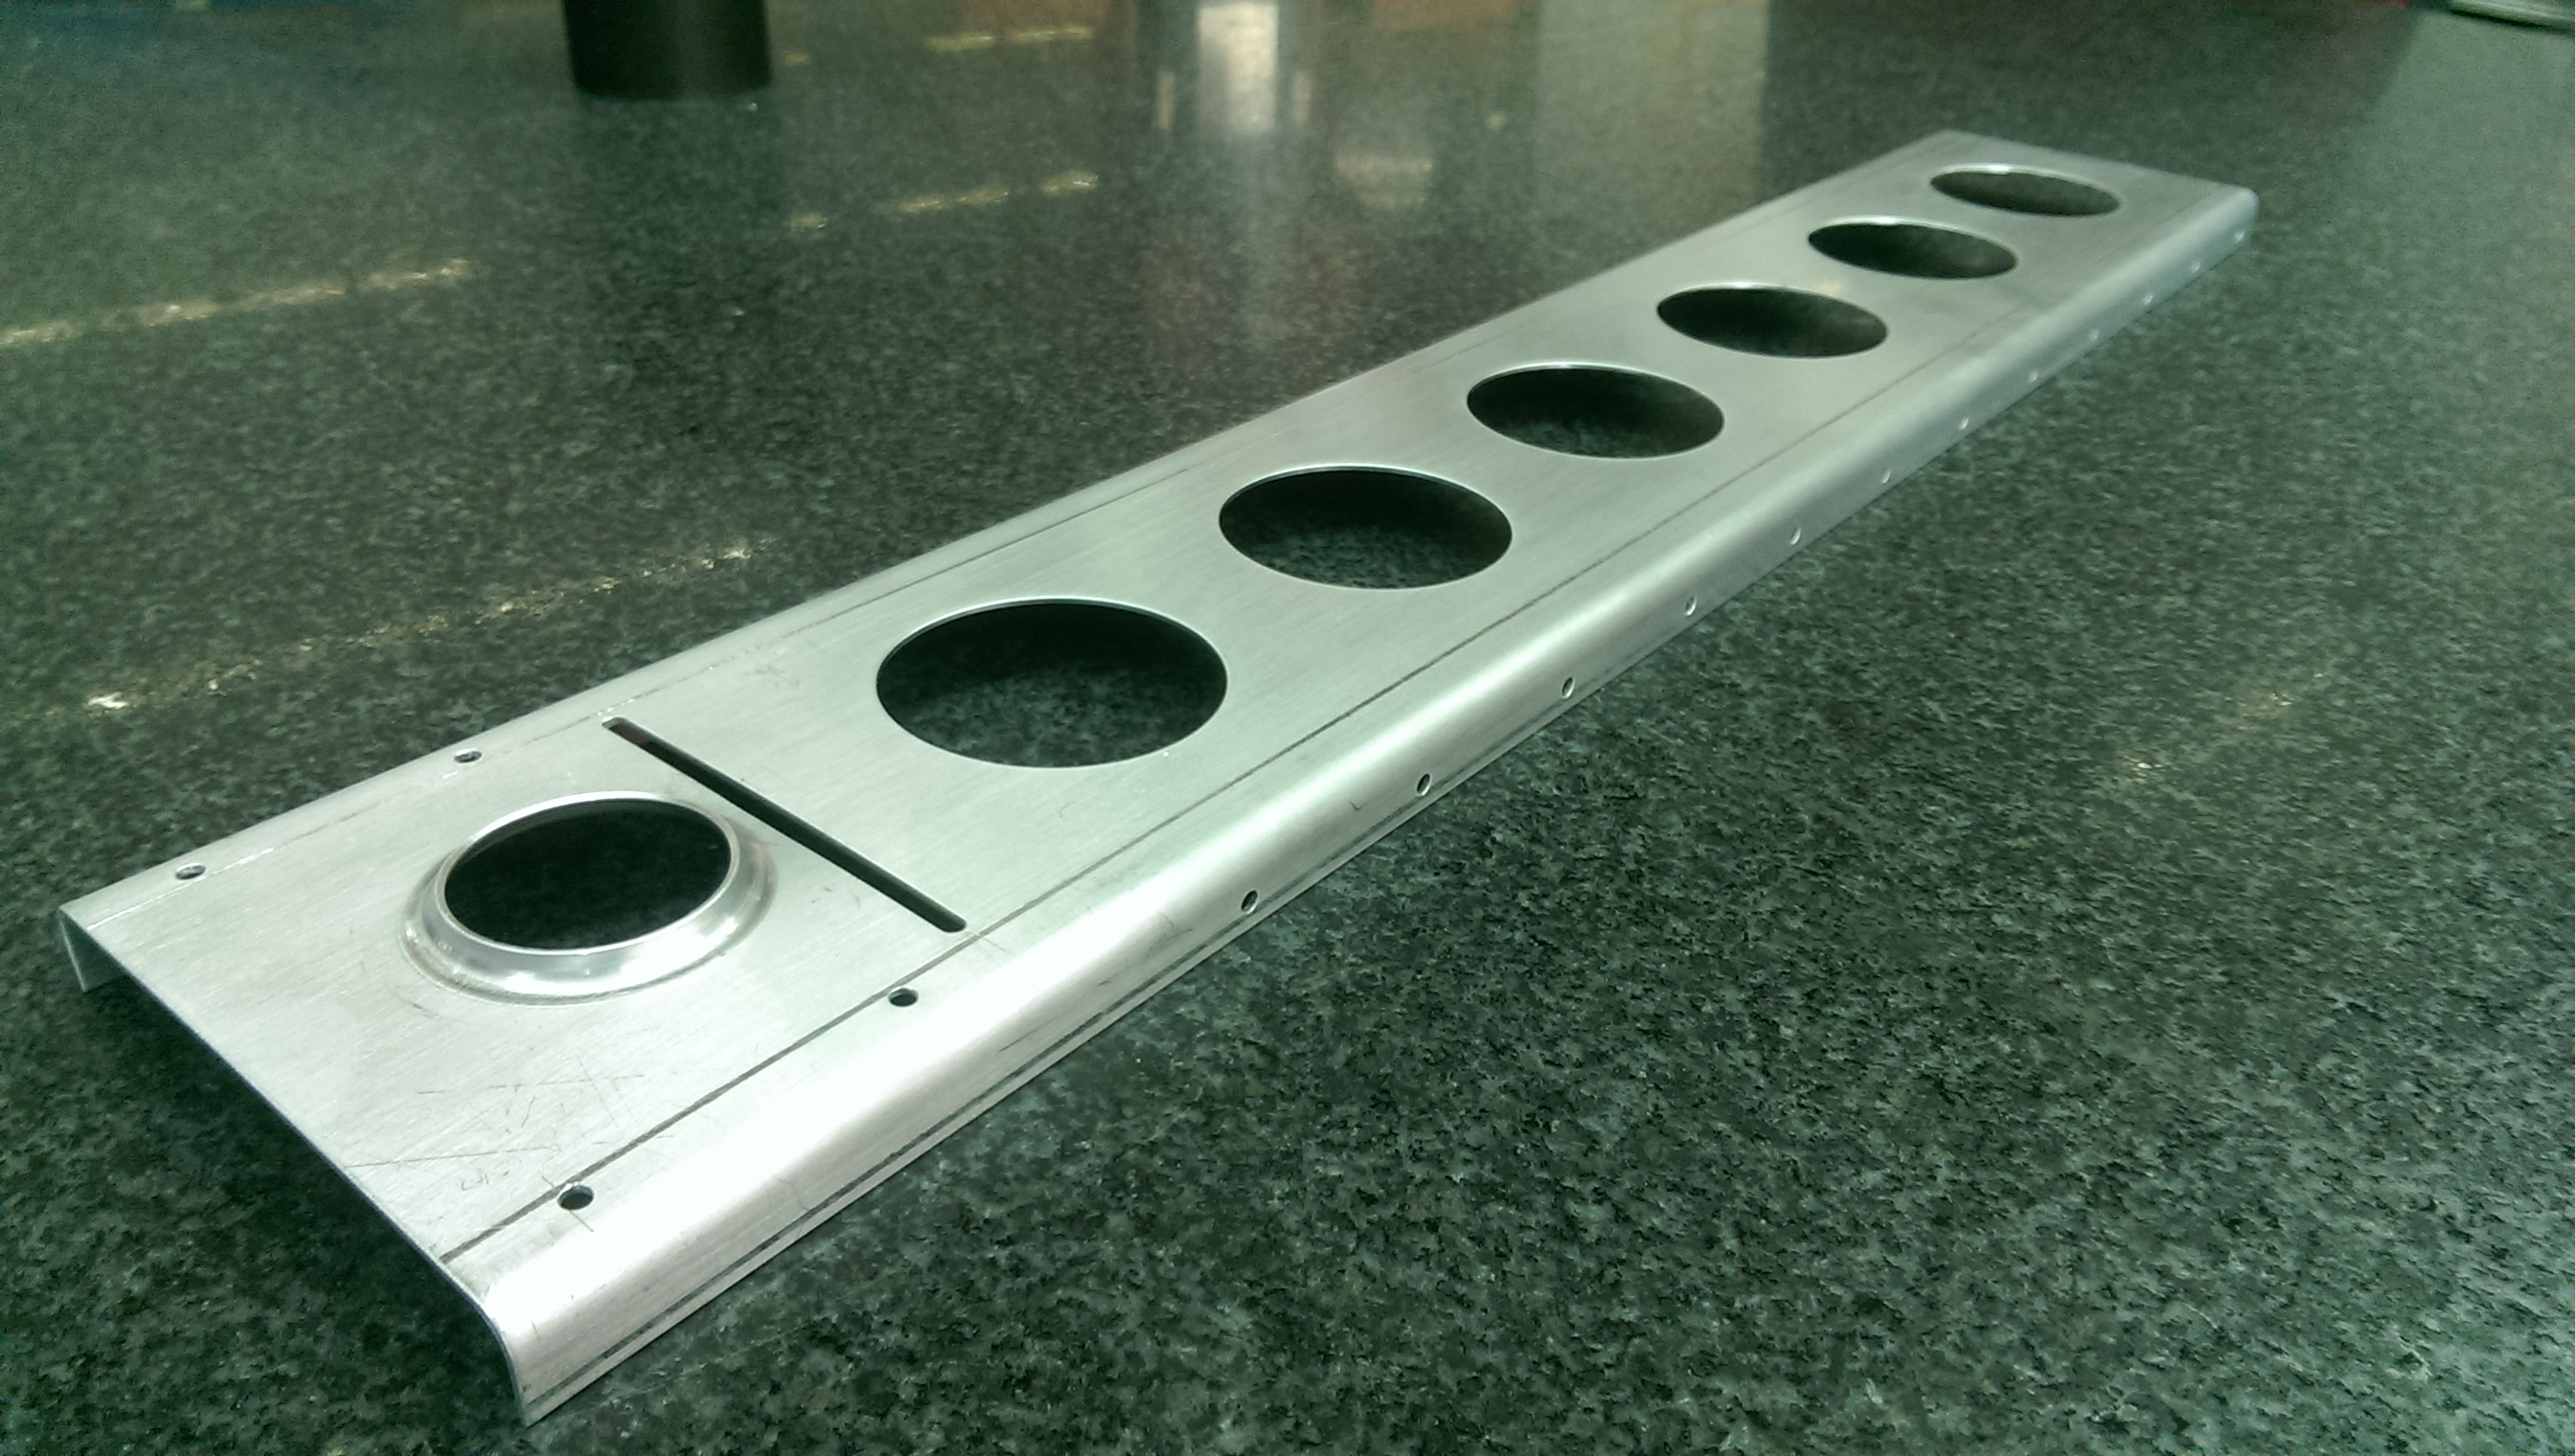
\includegraphics[width=0.5\textwidth]{fig/IMAG0364.jpg}
	\caption{Seitenteil Balllager}
	\label{fig:Seitenteil Balllager}        
\end{figure}

\subsubsection{Ballager}
Das Balllager dient als Grundstruktur, an welcher der Ballnachschub und der Motor befestigt sind. Gelagert werden die Bälle im Inneren des quadratischen Querschnittes. Die Halterungen des Motors werden jeweils auf beiden Aussenseiten des vorderen Endes befestigt. Damit das Stahlband des Ballnachschubs optimal aufgewickelt werden kann, werden die herausstehenden Enden der Nieten mit Aluminiumleisten abgedeckt.

\subsubsection{Ballnachschub}
Der Ballnachschub besteht im Wesentlichen aus einer Trommel, einem Stahlband und einem Servomotor. Das Stahlband wird im Inneren des Balllagers um die Bälle herum ausgelegt. Durch das Aufwickeln des Bandes auf die Trommel werden die Bälle Richtung Beschleunigungsrad gezogen. Der Antrieb erfolgt durch einen umgebauten Servomotor, welcher mittels Zahnriemen mit der Welle der Trommel verbunden ist.
\paragraph{Auslegung}
Als Servo dient ein HS85MG der Firma Hitec. Dieses ist wie folgt spezifiziert: 
\begin{table}[h!]
	\centering
	\begin{zebratabular}{lll}
		\rowcolor{gray}
		Parameter &
		Wert bei 4.8\si{\volt} &
		Wert bei 6.0\si{\volt} \\
		Stellgeschwindigkeit (60\si{\degree}) &
		0.16\si{\second} &
		0.14\si{\second} \\
		Drehmoment &
		3.0\si{\kilogram\per\centi\metre} &
		3.5\si{\kilogram\per\centi\metre} \\
	\end{zebratabular}
	\caption{Spezifikation Servomotor}
\end{table}
Dies ergibt folgende Spezifikationen für den sich daraus ergebenden DC Motor: 
\begin{table}[h!]
	\centering
	\begin{zebratabular}{lll}
		\rowcolor{gray}
		Parameter &
		Wert bei 4.8\si{\volt} &
		Wert bei 6.0\si{\volt} \\
		Stellgeschwindigkeit (60\si{\degree}) &
		62.5\si{\per\minute} &
		71.4\si{\per\minute} \\
		Drehmoment &
		0.3\si{\newton\metre} &
		0.35\si{\newton\metre} \\
	\end{zebratabular}
	\caption{Spezifikation DC Motor}
\end{table}

\subsubsection{Drehvorrichtung}
Die Drehvorrichtung dient zur horizontalen Ausrichtung der 
Abschussvorrichtung. Um eine genaue Positionierung und ausreichende Stabilität 
zu ermöglichen, wurde ein Zahnrad durch zwei 
Axial-Rillenkugellager auf einer Grundplatte verspannt. Die Ausrichtung wird 
durch einen Schrittmotor mit dem direkt verbundenen, kleineren Zahnrad 
eingestellt. Einen guten Bodenkontakt garantieren an der Unterseite der Füsse angeklebte Gummimatten.

\paragraph{Auflösung}
Der Schrittmotor benötigt 200 Schritte für eine Umdrehung. Er wird mit 1/128 
Mikrosteps angesteuert. Die Übersetzung beträgt 1:4.8. Daraus ergibt sich 
folgende Auflösung: 
\[ 200 \cdot 128 \cdot 4.8 = 122'880 \frac{\text{Schritte}}{\text{Umdrehung}}  \]
\[ \frac{360^\circ}{122'880} = 0.0029296875 \frac{^\circ}{\text{Schritt}} 
= 0.17578 \frac{'}{\text{Schritt}} = 10.547 \frac{''}{\text{Schritt}}
\rightarrow 341.33 \frac{\text{Schritte}}{^\circ}\]

\subsubsection{Motor}
Der Motor wird als Eigenkonstruktion ausgeführt. Der Läufer wird auf einer CNC-Fräsmaschine gefräst, wobei dieser sogleich als Felge des 
Beschleunigungsrades dient. Aufgrund der magnetischen Eigenschaften muss zusätzlich ein Stahlring eingepresst werden.

\subsubsection{Turm}
Der Turm dient als Verbindungselement des Balllagers mit dem grösseren 
Zahnrad der Drehvorrichtung. Ausgeführt wird die gesamte Konstruktion aus Aluminiumblech. Der Platz im Inneren wird zum Verstauen der 
Elektronikkomponenten verwendet. Hierfür wird die vordere Abdeckplatte statt mit Nieten, mit Schrauben befestigt.

\clearpage
\subsection{Herstellung mechanische Komponenten}
Die konzeptionellen CAD-Zeichnungen werden ab Semesterwoche 2 weiter ausgearbeitet, abgewickelt und die Fertigungszeichnungen erstellt. Hierbei müssen hauptsächlich Details wie Bohrungen für die Nieten angebracht und einige konstruktive Anpassungen vorgenommen werden. 

Ab Semesterwoche 3 können die ersten Teile an der Fräsmaschine im Elektrotechniklabor produziert werden, wobei parallel  hierzu die restlichen Komponenten am CAD fertiggestellt werden.
Um die gebogenen Innenkanten der Aussparungen zu realisieren, werden die gefrästen Blechteile mit einer Handpresse und eigens hierfür hergestellten Werkzeugen gefertigt.

In Semesterwoche 4 werden die Grundplatte zur Fertigung an der HSLU in Auftrag gegeben.

In Semesterwoche 5 werden zusätzlich einige Teile zum spanenden Herstellen, sowie zum 3D-Drucken in Auftrag gegeben. Ebenfalls wird eine Rohmaterialbestellung abgegeben.

Die in Auftrag gegebenen Teile können in Semesterwoche 6 abgeholt werden, wobei das  Rohmaterial fälschlicherweise aus Stahl, anstatt aus Aluminium, bestellt wurde. Eine neue Bestellung des richtigen Rohmaterials wurde abgesetzt.

In Semesterwoche 7 können die bestellten Teile sowie die zum biegen extern in Auftrag gegebenen Teile abgeholt werden. Des weiteren wird mit dem Zusammenbau der einzelnen Komponenten begonnen. Aufgrund eines beim Biegen entstandenen Verzugs einzelner Bauteile und einiger konstruktiver Ungenauigkeiten müssen diverse Bohrungen durch feilen nachgebessert werden. Durch Niethefter kann die Konstruktion bis zum endgültigen Vernieten aufgebaut werden.

\begin{figure}[h!]          
	\centering             
	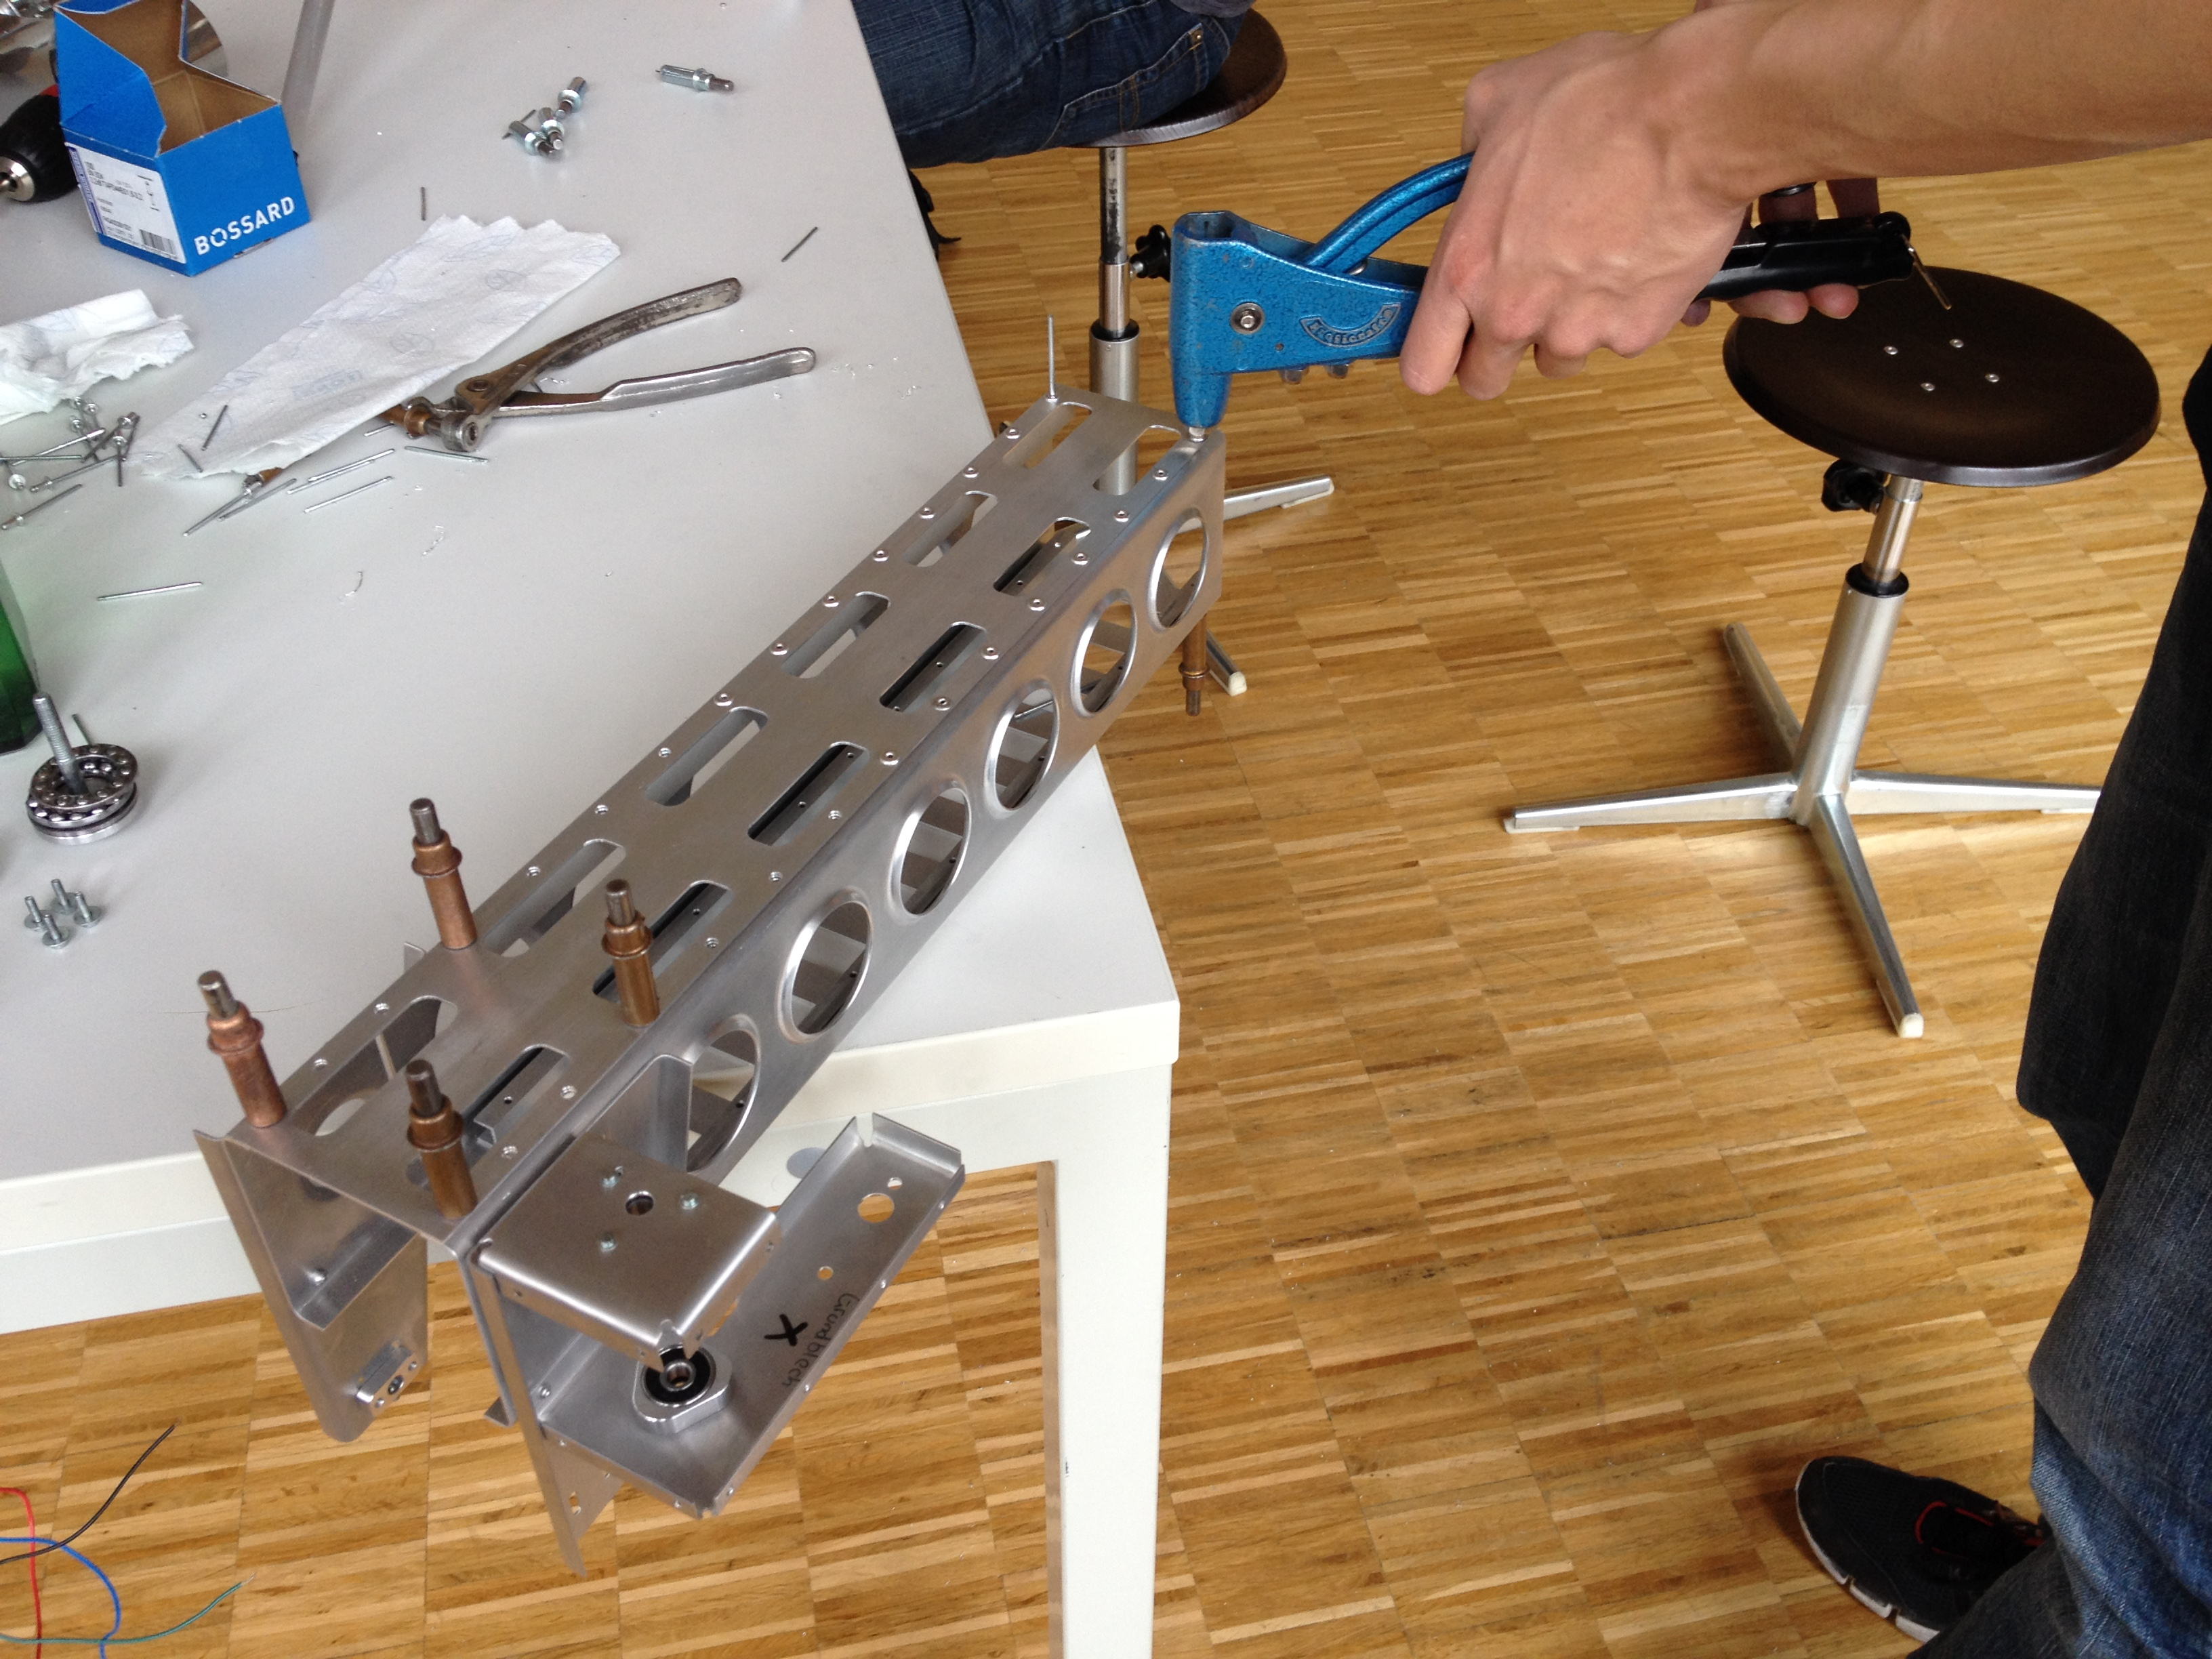
\includegraphics[width=0.5\textwidth]{fig/IMG_2290.JPG}
	\caption{Zusammenbau Balllager}
	\label{fig:Zusammenbau Balllager}        
\end{figure}

\begin{figure}[h!]          
	\centering             
	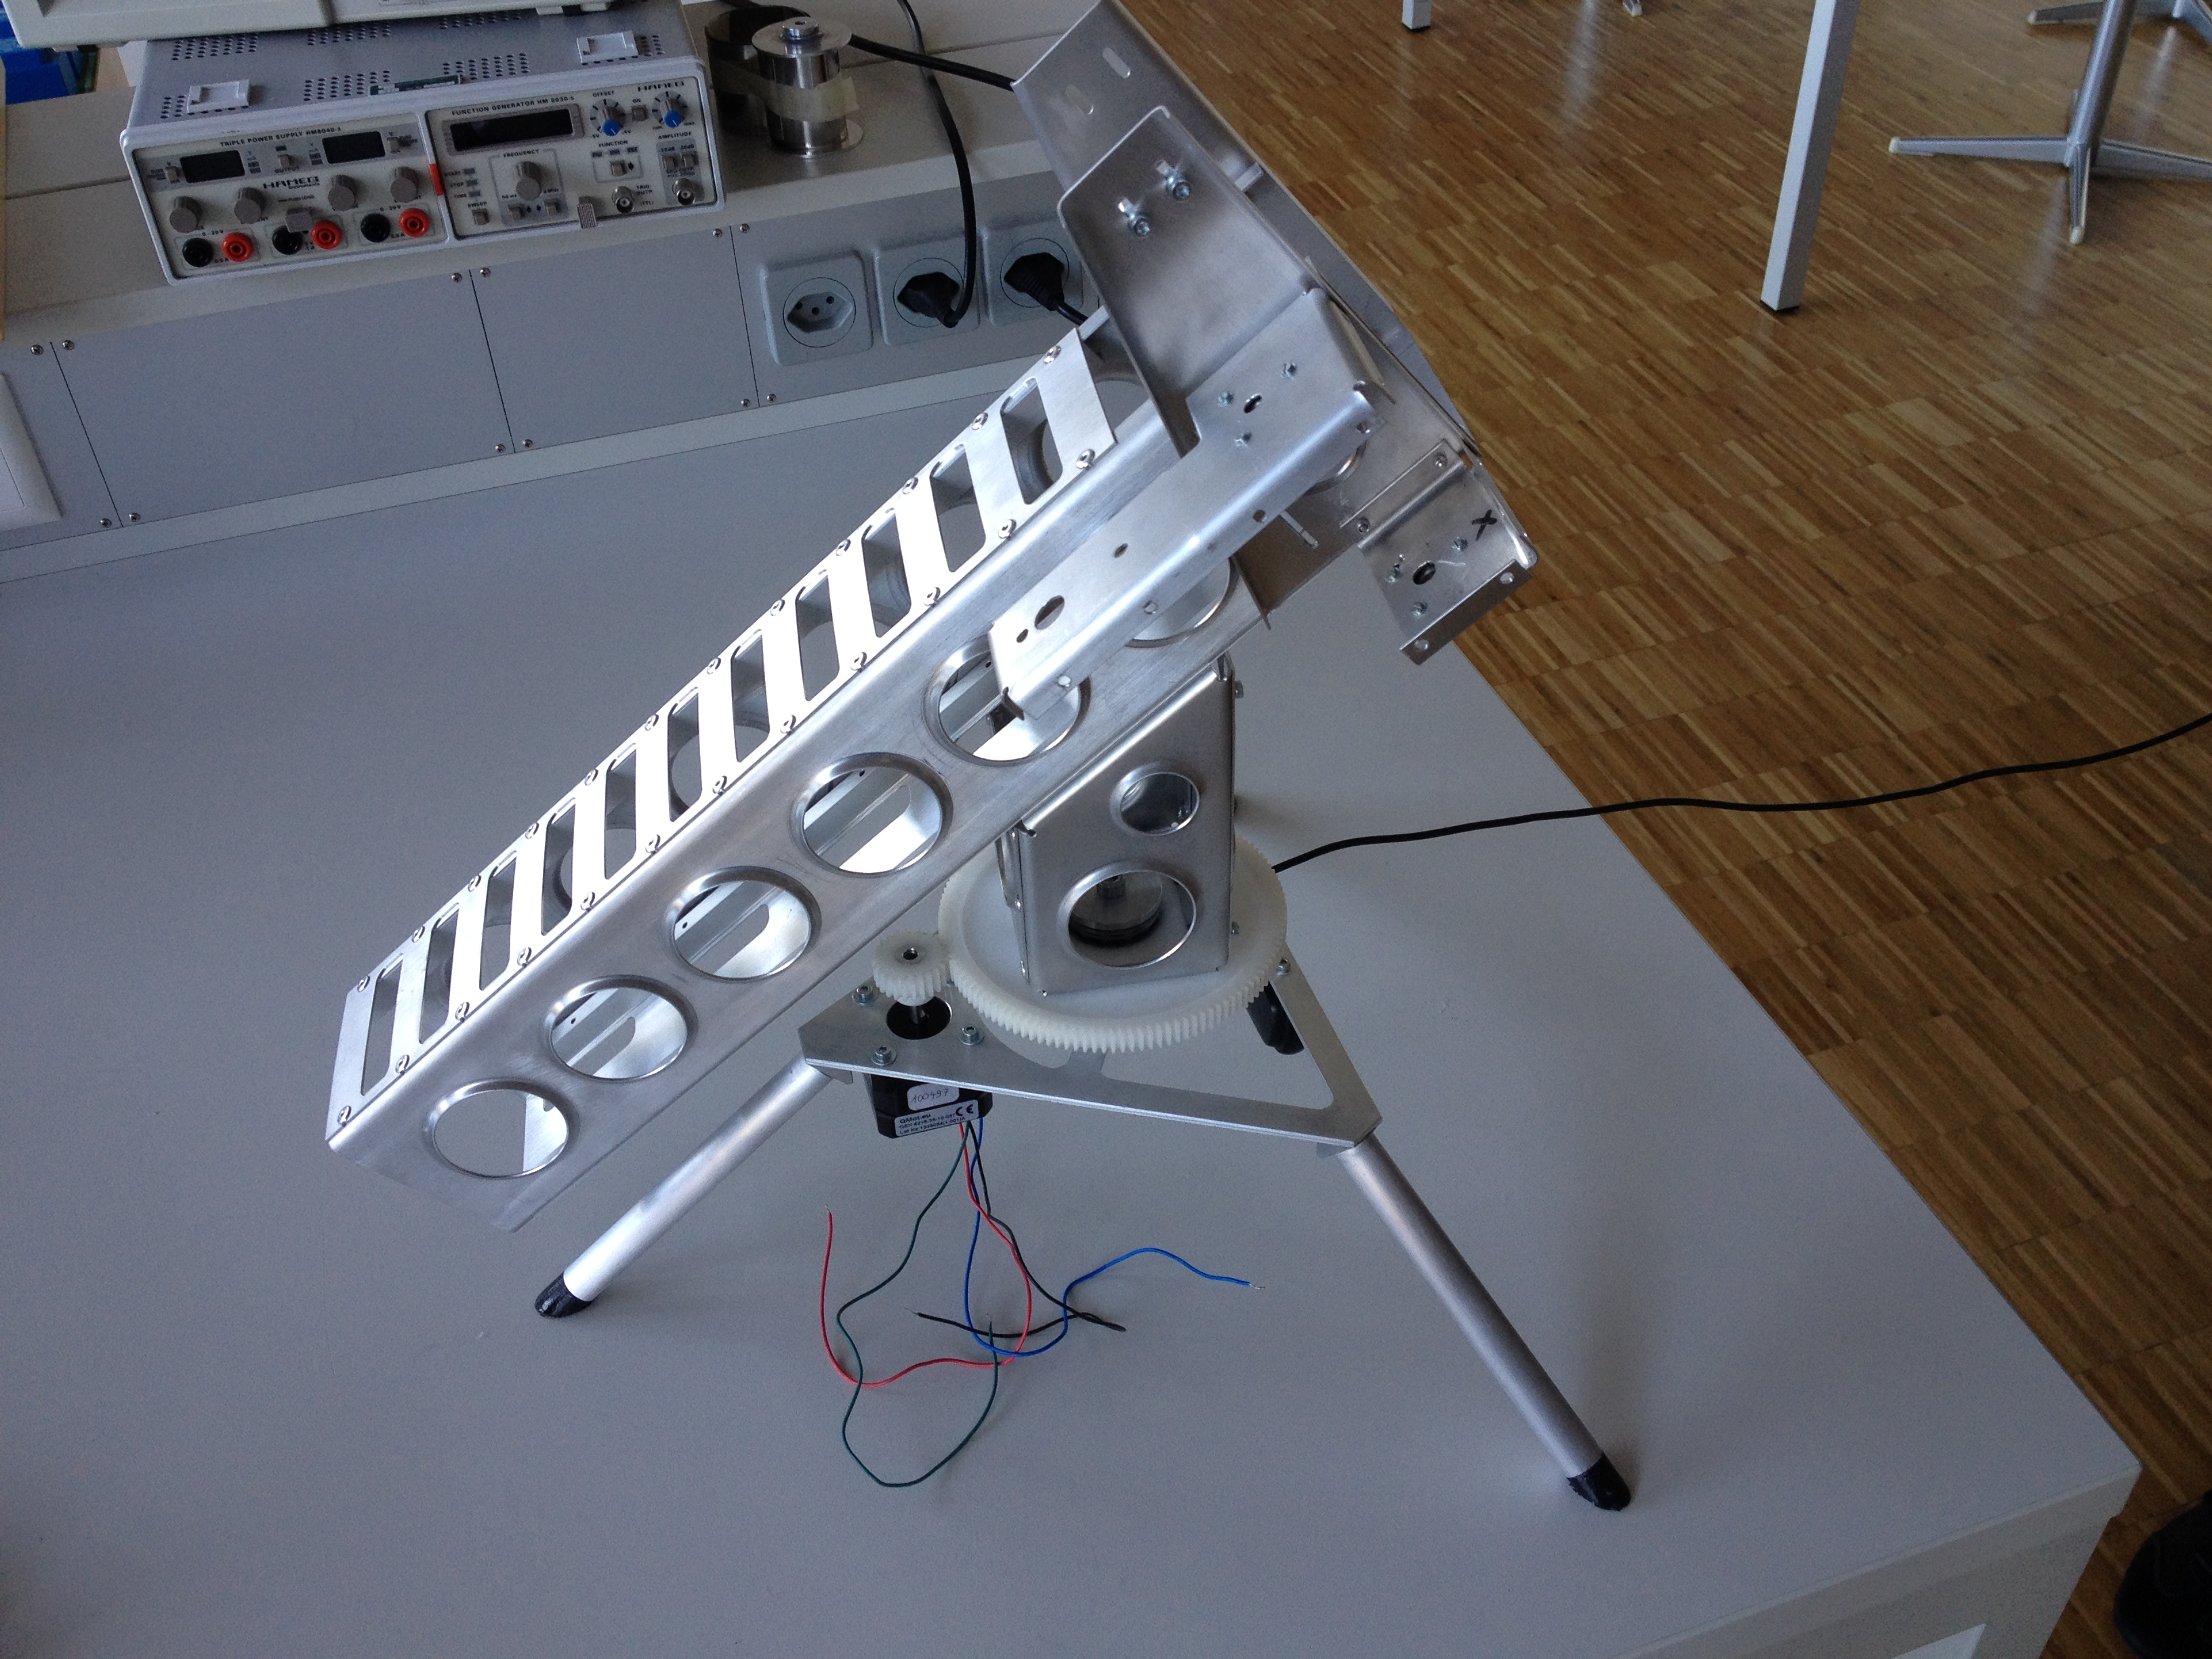
\includegraphics[width=0.5\textwidth]{fig/IMG_2303.JPG}
	\caption{Unvollständiger Aufbau}
	\label{fig:Unvollständiger Aufbau}        
\end{figure}

\subsubsection{Balllager}
Anhand der Erfahrungen erster Testläufe wird entschieden, keine Verstärkung an der Unterseite des vorderen Endes anzubringen. Diese Verstärkung hätte eine zu starke Durchbiegung des Blechs beim Abschuss der Bälle verhindert.
\subsubsection{Ballnachschub}
Beim Zusammenbau wird festgestellt, dass die Welle der Trommel einen zu grossen Durchmesser hat und daher mit Hilfe einer Handbohrmaschine und gewöhnlichem Schleifpapier auf das gewünschte Mass geschliffen werden muss.
\subsubsection{Drehvorrichtung}
Um weiteres Gewicht einzusparen wird die bereits hergestellte Grundplatte auf die halbe Höhe überfräst.

\begin{figure}[h!]          
	\centering             
	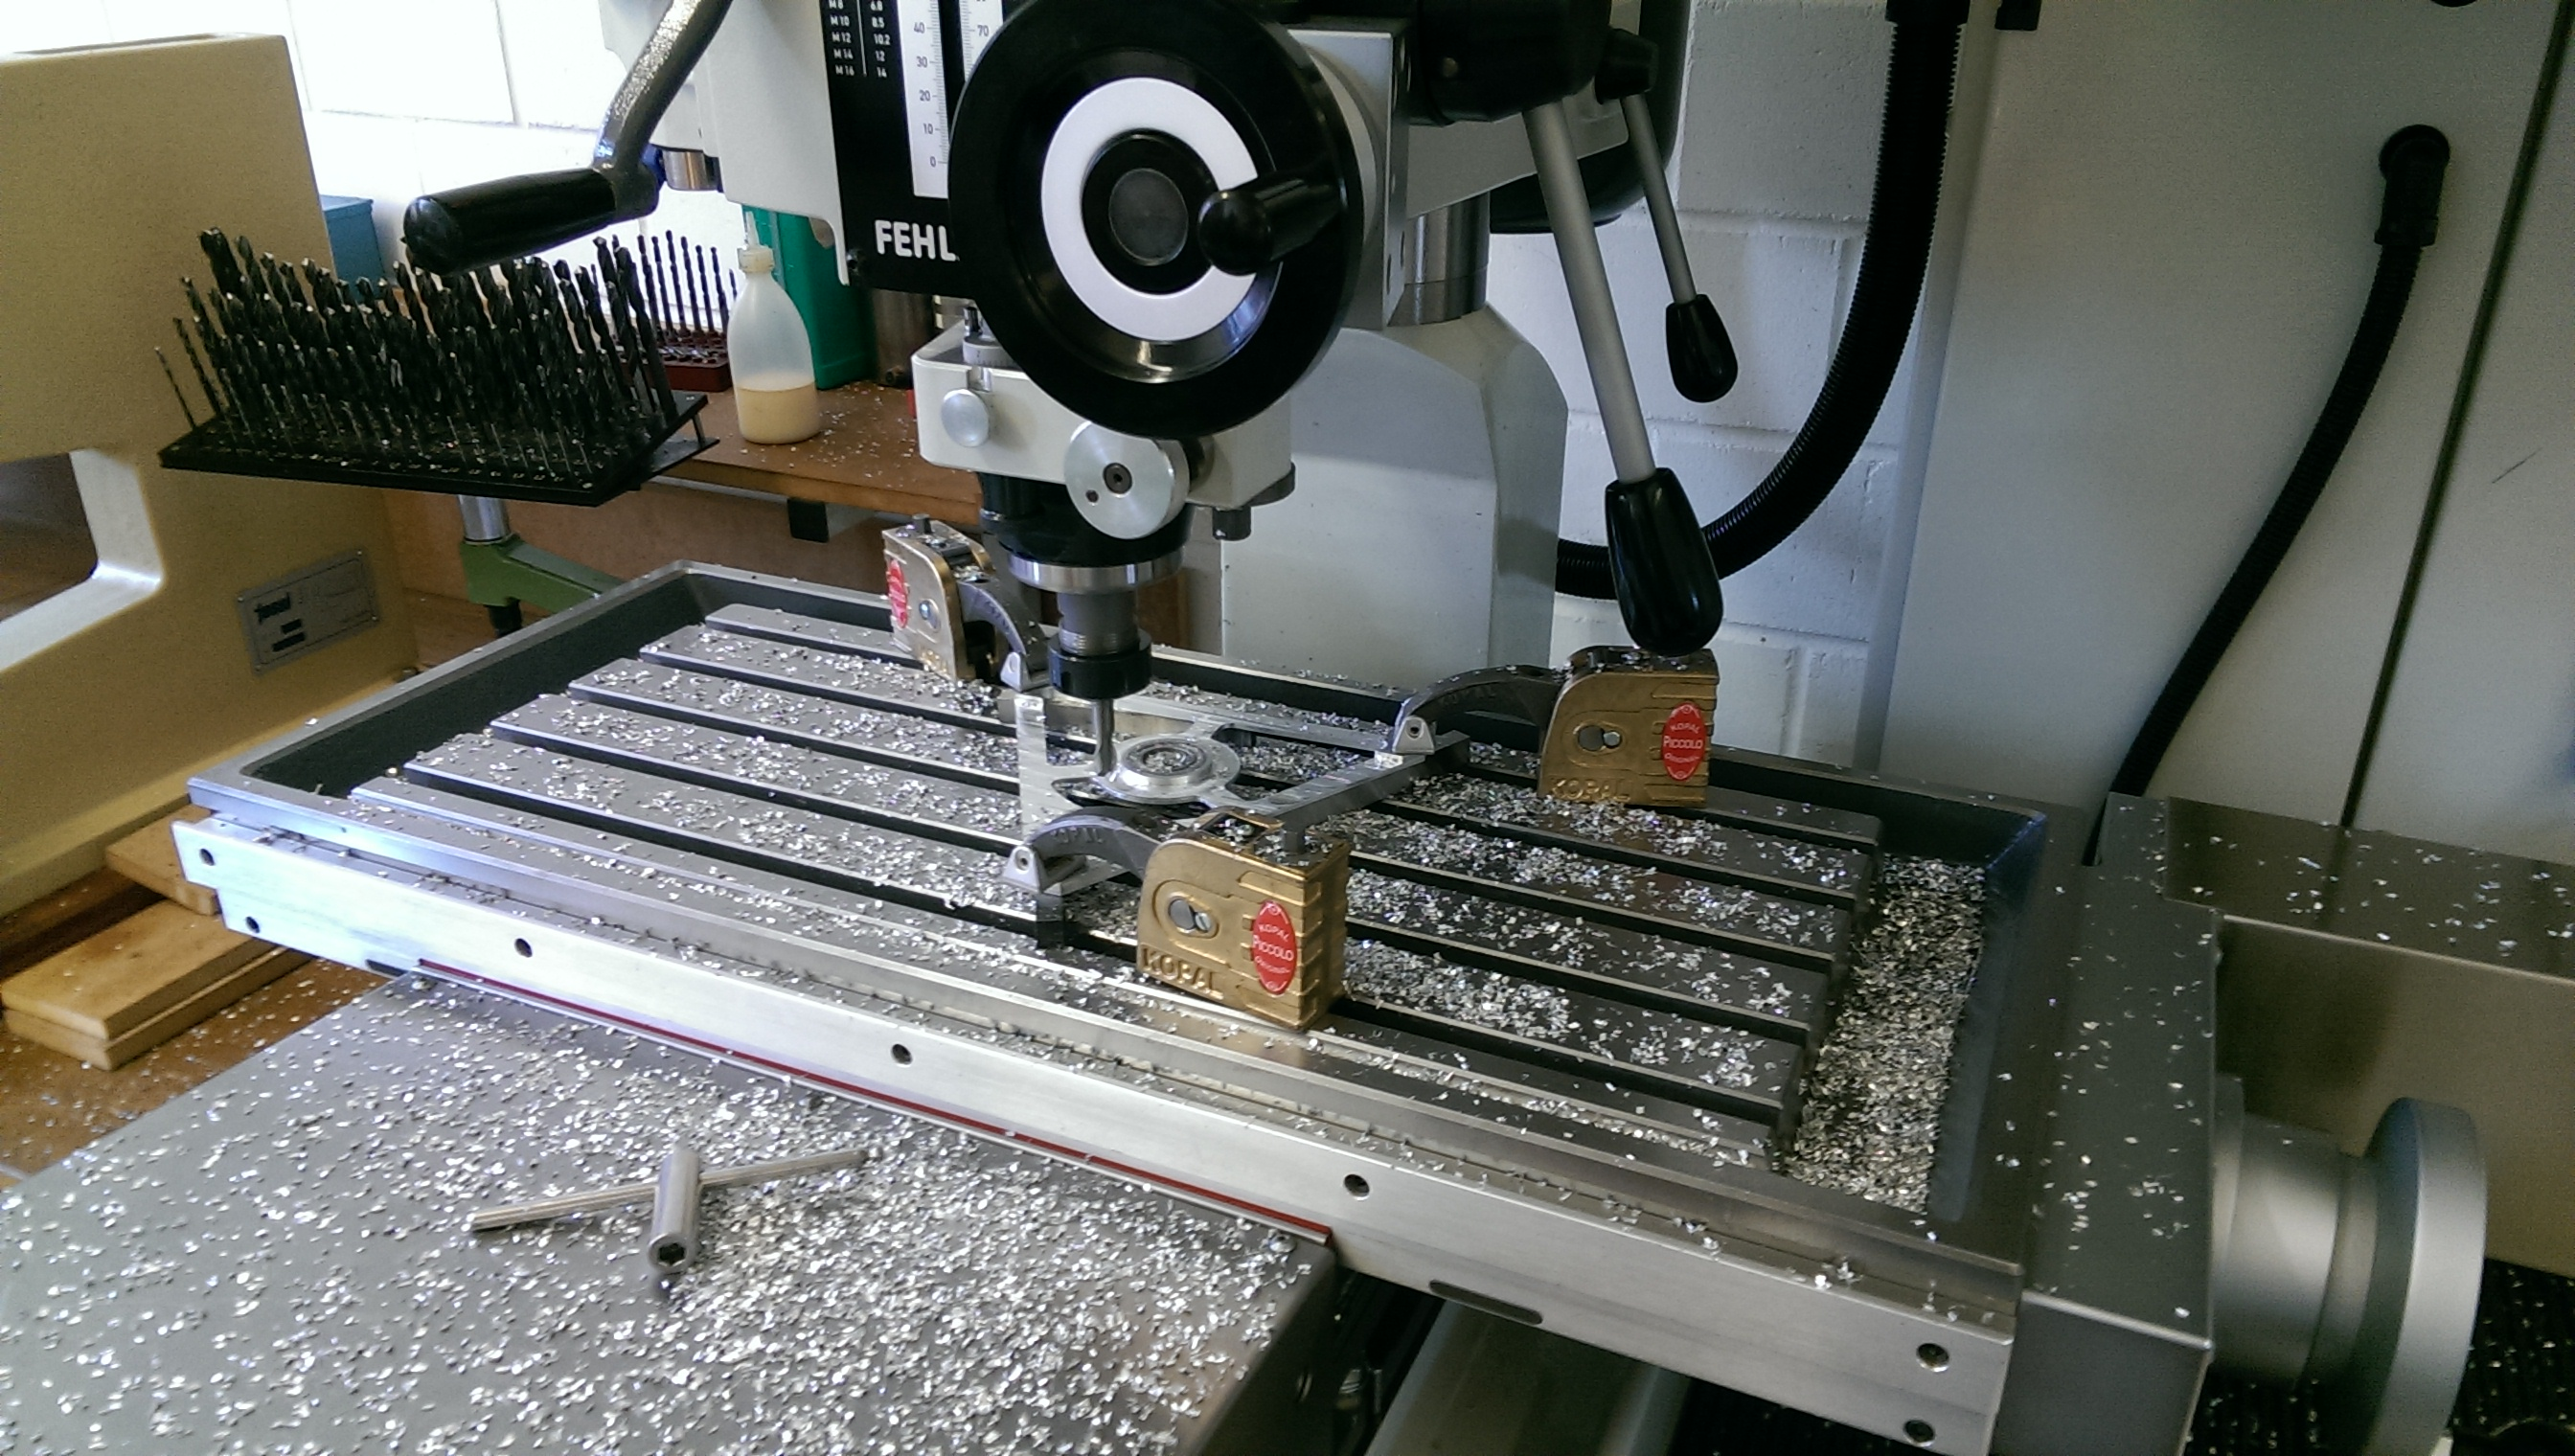
\includegraphics[width=0.5\textwidth]{fig/IMAG0357.jpg}
	\caption{Überfräsen der Grundplatte}
	\label{fig:Grundplatte fräsen}        
\end{figure}

\subsubsection{Motor}
Sämtliche Magnete werden von Hand eingesetzt und mit Zweikomponentenklebstoff befestigt. Der Stator wird aus gebrauchten Floppydisk-Laufwerken ausgebaut, neu gewickelt und an einer gefrästen Halterung befestigt.

Beim Zusammenbau wurde bemerkt, dass die Langlöcher der Motorenhalterung zu kurz ausgeführt wurden um einen guten Anpressdruck der Bälle zu ermöglichen. Daher werden diese durch feilen verlängert.

\subsubsection{Turm}
Die Muttern werden auf der Innenseite des Turms mit Zweikomponentenklebstoff angebracht.

\begin{figure}[h!]          
	\centering             
	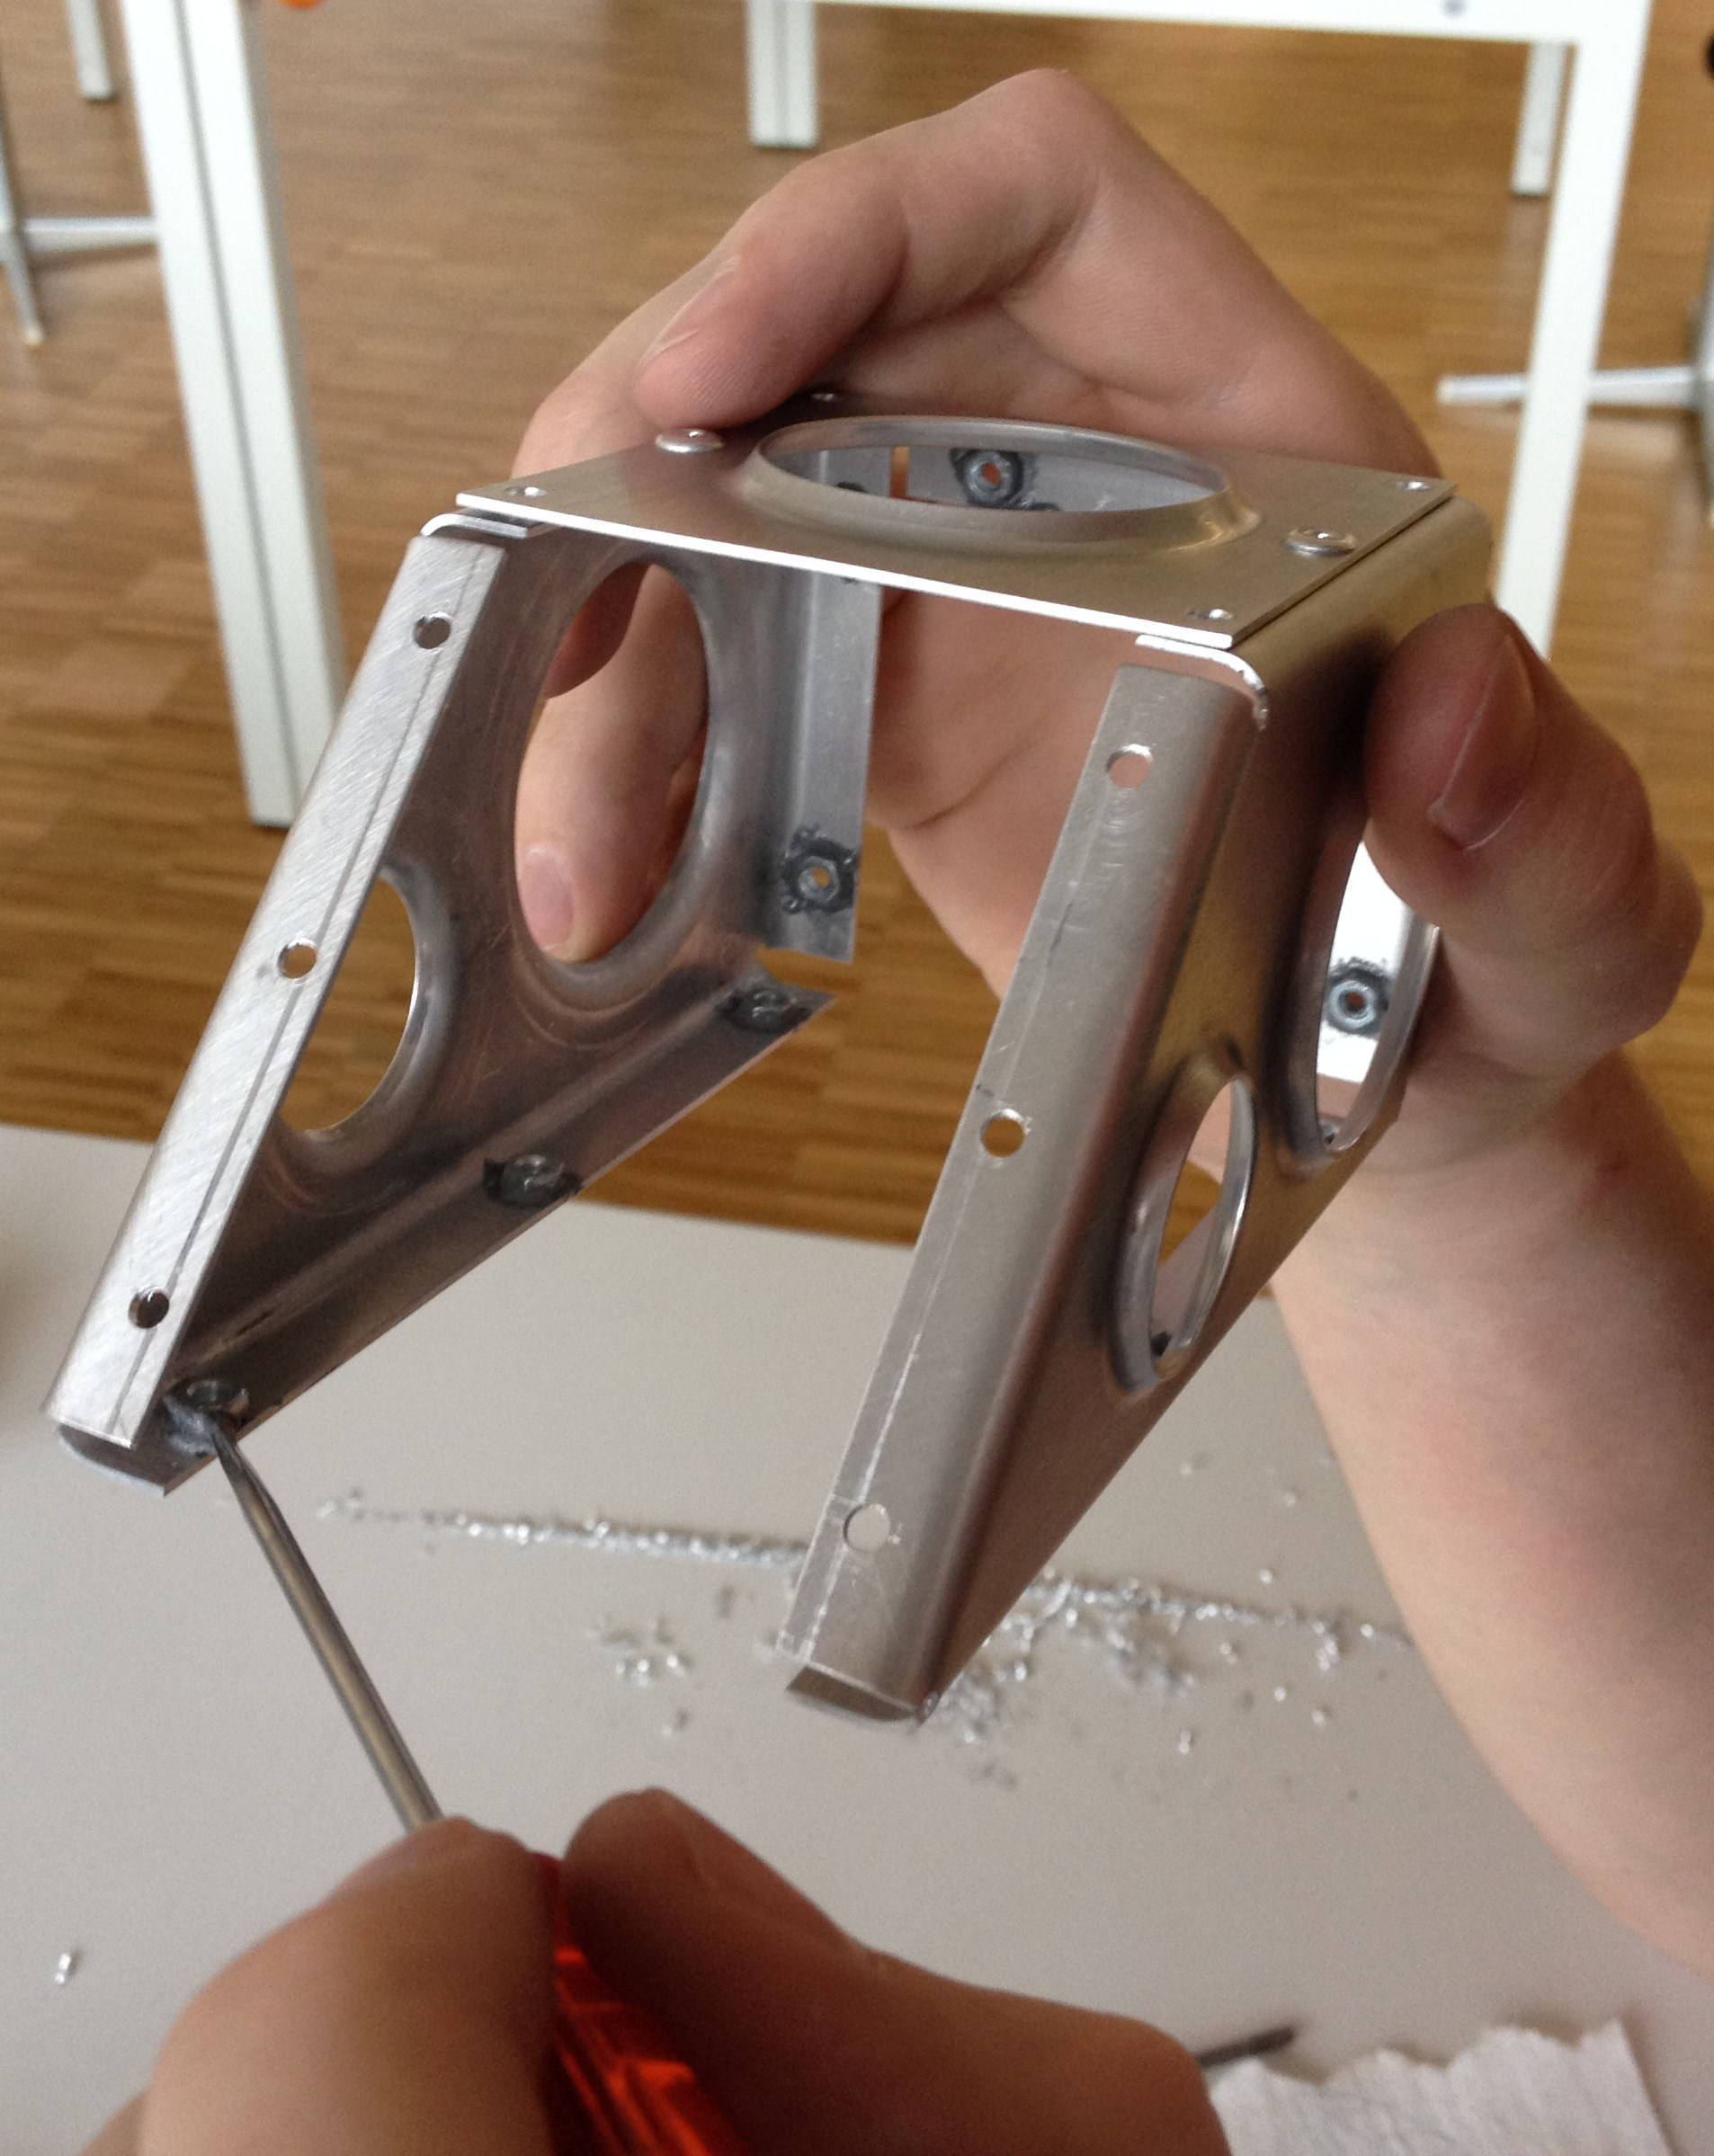
\includegraphics[width=0.3\textwidth]{fig/IMG_2292.JPG}
	\caption{Kleben der Muttern}
	\label{fig:Muttern Kleben}        
\end{figure}


